\documentclass{mwart}
%\usepackage{polski}
%\usepackage[polish]{babel}
\usepackage{amsfonts}
\usepackage{indentfirst}
\usepackage[utf8]{inputenc}
\usepackage{amsthm}
\usepackage{multirow}
\usepackage{amsmath}
\newtheorem{tw}{Twierdzenie}
\newtheorem{df}{Definicja}
\newtheorem{zd}{Zadanie}
\newtheorem{zdt}[zd]{Zadanie*}
\title{Zestaw 8}
\usepackage{Sweave}
\begin{document}
\Sconcordance{concordance:Zestaw8.tex:Zestaw8.Rnw:%
1 14 1 1 0 74 1 1 2 1 0 1 1 1 2 2 1 1 9 6 0 1 8 6 0 1 4 2 0 1 1 4 0 1 2 %
1 1}

\maketitle

\begin{zd}
	Oblicz
	\begin{itemize}
		\item $\mathbb{P}(W_s < W_t)$,
		\item $\mathbb{P}(0 < W_2 < W_3)$
		\item $\mathbb{E}W_1W_2^2$
		\item $\mathbb{E}\left(W_2^2(W_3 - W_1)\right)$.
	\end{itemize}
\end{zd}

\begin{zd}
Niech $W$ będzie procesem Winera z wariancją $9$. Oblicz
\begin{itemize}
\item $\mathbb{P}(W_2 \leq 15)$,
\item $Var(3W_2-2W_5)$,
\item $\mathbb{P}(W_2-2W_3\leq 4)$,
\item $\mathbb{P}(|W_4-W_2|> 10)$,
\item $Var(3+W_4-2W_2+W_3)$,
\item $Cov(3+W_4-2W_2, 5-W_3)$.
\end{itemize}
\end{zd}

\begin{zd}
Niech $W$ będzie procesem Wienera na odcinku $[0, T]$ i niech proces $X$ będzie określony jako $X_t = tW_t - \int_0^tW_sds$. Czy proces $X$ jest martyngałem względem filtracji naturalnej procesu Wienera?
\end{zd}

\begin{zd}
	Określmy następujący proces (most Browna)
	\begin{displaymath}
		B_t = W_t - tW_1, \ t\in[0,1].
	\end{displaymath}
	Sprawdź, czy jest on martyngałem względem swojej filtracji naturalnej i znajdź jego funkcję kowariancji.
\end{zd}

\begin{zd}
Procesem Wienera z dryftem $\mu$ i wariancją $\sigma^2$ nazywamy proces $X_t = \mu t+ \sigma W(t)$.
\begin{itemize}
\item Wykaż, że proces $X$ ma niezależne i stacjonarne przyrosty.
\item Znajdź rozkład $X(t)$.
\item Sprawdź, czy proces $X$ jest martyngałem.
\end{itemize}
\end{zd}

\begin{zd}
	Pokaż, że proces określony jako $Z_t = \sqrt{t}N(0,1)$ nie jest procesem Wienera.
\end{zd}

\begin{zd}
	Sprawdź, czy następujące procesy są procesami Wienera:
	\begin{itemize}
		\item $-W_t$,
		\item $c^{-1/2}W_{ct}$, $c>0$,
		\item $Y_t = tW_{1/t},\ t> 0$ i $Y_0 = 0$,
		\item $W_{T+t} - W_T, \ T > 0$.
	\end{itemize}
\end{zd}

\begin{zd}
Niech $(W_t)_{\{t \geq 0\}}$ będzie procesem Winera, $(B_t)_{t\in [0, 1]}$ będzie mostem Browna i niech $Z$ będzie zmienną losową o standardowym rozkładzie normalnym. Udowodnij
\begin{itemize}
\item $X_t = B_t+tZ$ jest procesem Winera na odcinku $[0, 1]$,
\item $X_t = (t+1)B_{t/(t+1)}$ jest procesem Wienera na odcinku $[0, \infty)$,
\end{itemize}
\end{zd}

\begin{zd}
Niech $W$ będzie procesem Winera. Znajdź postać funkcji gęstości zmiennej losowej $X = W(a) + W(b)$, gdzie $0 \leq a < b$.
\end{zd}



\begin{Schunk}
\begin{Sinput}
> library(tidyverse)
> library(foreach)
> steps <- 1000
> interval <- 1
> n_sim <- 10
> simulate_path <- function(steps, interval, simulation_nr = NA) {
+   dt <- sqrt(interval/steps)
+   increments <- rnorm(steps-1)
+   return(data.frame(simulation = rep(simulation_nr, length(steps)),
+                     values = cumsum(c(0, dt*increments)),
+                     time = seq(0, interval, length.out = steps)))
+ }
> plot <- function(data) {
+   data %>%
+   ggplot(aes(x = time, y = values, col = as.factor(simulation))) +
+   geom_step(size = 1) +
+   theme(legend.position = "none") +
+   labs(title = "Wiener proces")
+ }
> data <- foreach(n = 1:n_sim, .combine = rbind) %do% {
+   simulate_path(steps = steps, interval = interval, simulation_nr = n)
+ }
> plot(data)
\end{Sinput}
\end{Schunk}
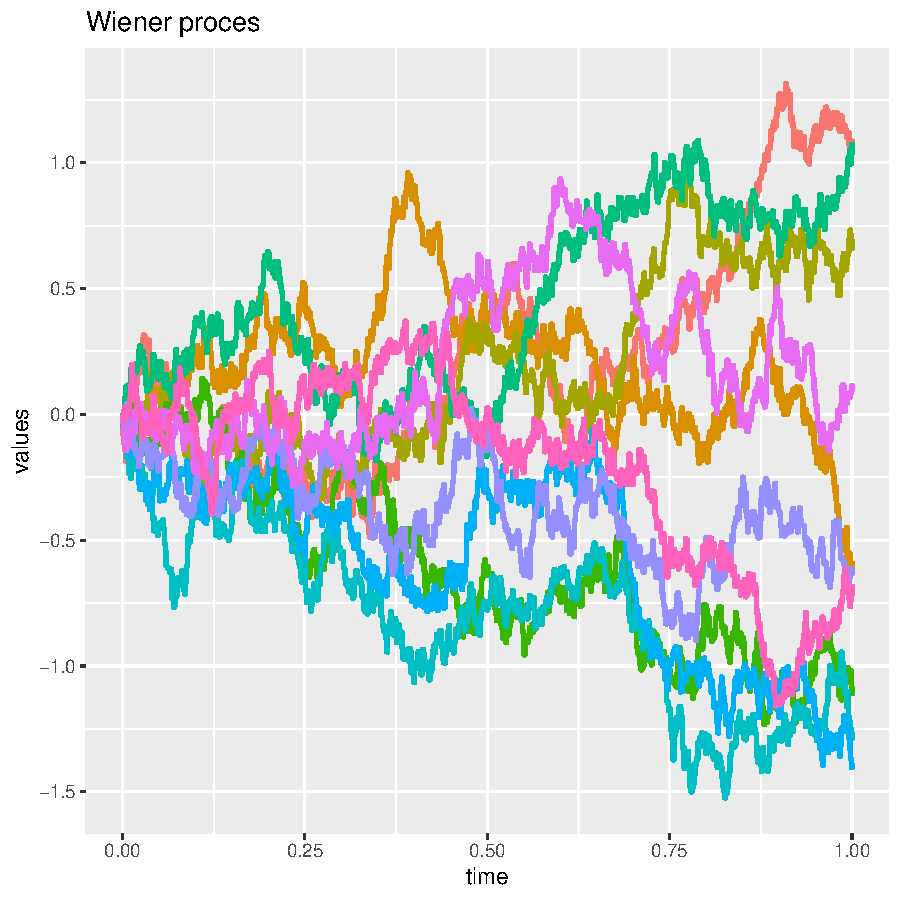
\includegraphics{Zestaw8-001}

\end{document}
